\chapter{Teletrabajo}\label{S:anexo_A}

Este anexo resume los conceptos básicos, estado del arte actual tanto desde el punto de vista legal, funcional o práctico relacionado con el “teletrabajo”. El principal objetivo es diferenciar nuestro caso de estudio del resto de casuísticas.

\section{Contexto Semántico}

¿Que es el teletrabajo o home office? ¿Es lo mismo que el trabajo en remoto?

Comencemos definiendo el significado de las palabras, la interacción entre ellas y el uso técnico que entendemos al usarlas. Teletrabajo, significa trabajar a distancia (“tele-” prefijo griego lejos),  “home office” es el término en inglés para indicar trabajar desde casa y “trabajar en remoto” indica que el trabajador realiza su tarea fuera de la oficina principal, es decir, de manera virtual.

\begin{figure}[htb]
\begin{center}
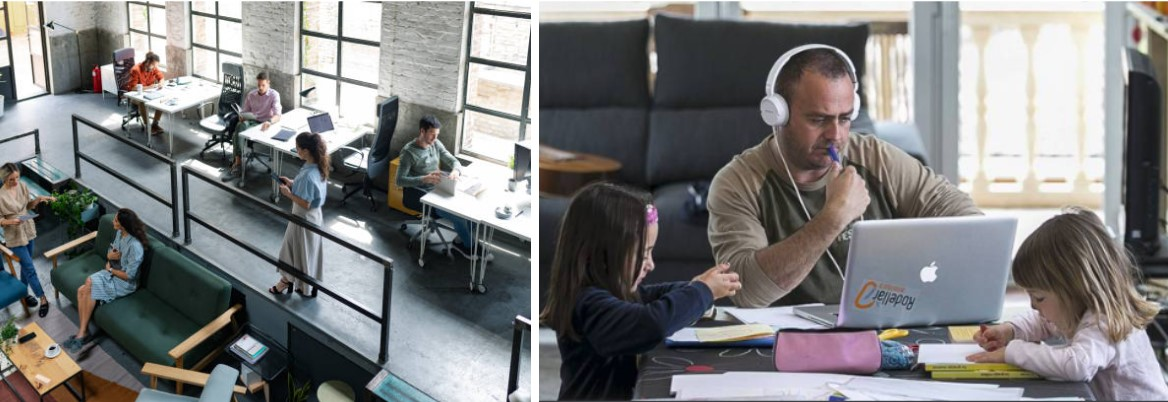
\includegraphics[width=1\textwidth]{./figuras/coworking_vs_homeoffice}
\caption{Coworking\cite{i_coworking} vs home office\cite{i_family}}
\label{F:coworking_vs_homeoffice}
\end{center}
\end{figure}

Aunque estas palabras son similares su uso técnico tiene diferencias significativas e implicaciones legales diferentes. Hemos de separar conceptualmente 3 visiones diferentes y complementarias, la organizativa a la hora de realizar el trabajo (grupo de trabajo), la situación física del trabajador y el carácter legal del trabajador.

Existen empresas que no tienen una sede física con oficina o tienen múltiples, las hay que mandan a sus trabajadores a las oficinas de sus clientes. En cualquiera de estos casos, estos trabajadores realizan el 100\% de su trabajo en remoto, puesto el grupo de trabajo no está reunido completamente en la misma oficina física, pero ninguno lo realiza desde su casa o consta como teletrabajo legalmente, puesto que se desplazan a la oficina que su compañía les indica.

Por otra parte, también existen muchas compañías que ofrecen flexibilidad horaria y la posibilidad de ‘teletrabajar’ dentro de su pack de conciliación. Que el trabajador pueda salir antes de la oficina y terminar un porcentaje de jornada desde casa (o cualquier otro lugar) con el fin facilitar su conciliación trabajo-vida familiar.

 Por último tenemos el caso de muchos trabajadores, especialmente mandos intermedios o especialistas cuyos proyectos con picos de trabajo realizan horas extras “trabajando desde casa”.

Desde el punto de vista técnico, \textbf{trabajar en remoto}, se refiere única y exclusivamente a realizar el trabajo (función dentro del grupo de trabajo) siendo exclusivamente dependiente de \textbf{medios virtuales}, es decir, el grupo de trabajo no está físicamente en contacto directo, no considera el lugar desde donde se realiza la actividad. Trabajar desde casa, o ‘\textbf{home office}’, indica que el trabajador dispone y realiza \textbf{un porcentaje significativo} (y mayoritario) de su trabajo en remoto, desde su vivienda habitual. Por último, \textbf{teletrabajar-legalmente} en España indica que el trabajador realiza más de un 30\% de su jornada laboral fuera de la oficina física de la empresa (ejemplo más 1.5 días a la semana o más de 2 horas 20 min diarias), o hasta un 50\% en contratos formativos.

Legalmente, el teletrabajo es voluntario, por lo tanto es un acuerdo fomentado por ambas partes. La empresa está obligada \cite{c_boe_teletrabajo} a firmar un contrato individual con el trabajador, donde se detallan los pormenores de la cesión de equipamiento y la compensación para los gastos ocasionados por el teletrabajo, así como los plazos, renovaciones y la posibilidad del cambio de dichas condiciones. Habitualmente suele quedar negociado dentro del convenio sindical, indicando que equipos o coworking designados y la cuantía mensual extra asociada a los gastos generados o con un presupuesto máximo preestablecido para nuevas incorporaciones. 

Esto en la gran  mayoría de casos suele plasmarse con “un acuerdo individual” basado en el convenio colectivo, usualmente con un portátil más todo aquel material que permiten llevar de la oficina a tu casa o una lista de elementos a comprar que la empresa te enviará a casa.


\section{Objetivo del teletrabajo}

Múltiples empresas han acabado implementado el teletrabajo, cada una por motivos diferentes\cite{c_work_remote_eurofound}, entre los principales objetivos y beneficios son los siguientes:
\begin{itemize}
    \item Productividad, principalmente relacionada con la mayor concentración de sus trabajadores en ambientes sin ruido ni interrupciones, junto a un uso más eficaz de su jornada al reducir el estrés de desplazarse a las oficinas y reducción de  tiempos perdidos o incidentes (atascos, meteorología, aglomeraciones ...).
    \item Flexibilidad extendida, principalmente focalizada en la conciliación familiar. “Un trabajador feliz” no solo es más productivo, es retener talento.
    \item Trabajadores des localizados, permite adquirir una plantilla no geo-localizada en una región local. Permite captar más talento, ya que el lugar de residencia no es requisito indispensable. Permite equilibrar salarial mente, aquellos lugares con rentas especialmente altas asociadas a grandes metrópolis.
    \item Reducción de costes asociados a la infraestructura física de las oficinas o servicios auxiliares de las mismas. Normalmente la reducción de costes en oficina física es superior a los acuerdos compensatorios de teletrabajo.
    \item Causa mayor, en algunas ocasiones eventos especiales, circunstancias climáticas-locales, situaciones político-sociales o causas médicas, no permiten la realización de la actividad laboral, siendo el teletrabajo la única opción.
\end{itemize}
Por otra parte requiere de una gestión o problemática asociada a la no interacción física, así como el \textbf{no uso} del “lenguaje no verbal” o comportamientos de grupos, difíciles de crear \textbf{sin un trabajo previo no remoto}. Por lo tanto existe las siguientes problemáticas:
\begin{enumerate}
    \item Mala gestión humana, recae en fuga de talento o bajada de productividad.
    \item Bajada generalizada de la creatividad y cohesión en equipos sin encuentros físicos.
    \item Requiere de una gestión jerárquica más directa y plana, así como una supervisión facilitada por ambos lados.
\end{enumerate}

\section{Histórico}
El trabajo en remoto existe hace décadas, especialmente desde la llegada del teléfono y los tele-operadores, pero para nuestra actual comprensión teletrabajar, está íntimamente ligado a trabajar con elementos tecnológicos que desde los años 90 permiten conectarse entre ellos y trabajar directamente con herramientas virtuales en constante comunicación.

Sin embargo ha sido una excepción de una élite muy especializada hasta la llegada de la banda ancha generalizada. No solo a sectores concretos sino también delimitado a regiones densamente pobladas y desarrolladas donde la conexión cumplía con los requisitos adecuados. 

\subsection{Pre pandemia}
Desde 2015 se observa un crecimiento significativo hasta el 5-15\%\cite{c_oecd_productividad_telework} en países desarrollados y la aparición de teletrabajo-des localizado especialmente en externalizaciones y freelance en países más competitivos salarial mente. Ambos casos se focalizan en una necesidad empresarial de obtener empleados cualificados, en un contexto de falta de personal y burbuja salarial.

Las principales características de estos trabajos son la flexibilidad familiar, la formación y la gratuidad de ciertos complementos con el fin del acceso a una mayor  disponibilidad de empleados cualificados que pueden realizar gran parte de su jornada laboral desde casa.

\subsection{Pandemia}
La pandemia covid-19 supuso en 2020-21 un verdadero experimento global que forzó por causas mayores\cite{c_boe_pandemia} el uso de teletrabajo en una gran parte de la población debido a las restricciones médicas. Aunque en algunas empresas especialmente de oficinas el teletrabajo ascendió por encima del 80\%, la realidad es que esta puesta acelerada donde destacaron la falta de medios, herramientas y organizaciones jerárquicas no preparadas para ello.
Desde mi punto de vista, los análisis y datos de este experimento social están muy sesgados por las circunstancias y recursos asociados a los empleados teletrabajando durante esos dos años. Especialmente llama la atención como grupos principalmente personas del sector tecnológico, sin cargas familiares y con unos recursos tecnológicos “semi-preparados” aumentaban significativamente la productividad y satisfacción. Mientras en otros con cargas familiares como niños o sin el adecuado espacio de trabajo lastraban su productividad y satisfacción. Por otra parte es complejo de evaluar, ya que muchas publicaciones son meramente estadísticas y no evalúan la formación y actuación de los mandos intermedios, ya que \textbf{gestionar empleados en remoto  es algo totalmente distinto}.

\subsection{Post Pandemia}
Actualmente dependiendo de qué país, pero especialmente de qué tipo de empresa, se están decidiendo cambios en el teletrabajo, especialmente de origen político-cultural, es decir, no especialmente racionales o justificables. Se han detectado patrones de comportamientos completamente opuestos, mientras hay empresas que insisten en una bajada de la productividad global, otras muestran una subida, generando tres tendencias:
\begin{itemize}
    \item Expansión y estandarización del trabajo en remoto, especialmente en empresas pequeñas, donde la cultura de objetivos y la digitalización favorece el debate ante una productividad mejorada o equilibrada con la reducción de costes asociados al teletrabajo. 

    \item Trabajo híbrido, especialmente en aquellas empresas de gran tamaño que han obtenido resultados contradictorios en sus diferentes grupos de trabajo. Intenta solventar las demandas de teletrabajo de sus trabajadores y la fuga de talento con la baja productividad o mala gestión de los mismos, con cuotas mínimas de días en oficina.

    \item Vuelta a la oficina, gran cantidad de empresas especialmente de gran tamaño, han optado por la vuelta irremediable a la oficina cambiando el teletrabajo, por flexibilidad, es decir inferior al 30\% de la jornada laboral.

\end{itemize}
Interesante es el colapso de servicios, principalmente en empresa o entes públicos, cuyas productividades ya eran bajas previamente a la pandemia,  han colapsado ante el teletrabajo favorecido por la administración, ya sea por una productividad aún menor o una falta de medios, organización o la falta de atención pública adecuada, parece estar destinada como ejemplo de cómo no implementar el teletrabajo.

\subsection{Opinión Personal}
Primero de todo he de indicar que aunque soy partidario del teletrabajo 100\% remoto, aceptó ampliamente la necesidad de 1 o más días en oficina y me interesa especialmente destacar ciertos puntos que no están en el actual debate de “teletrabajo vs oficina”.

El teletrabajo es una herramienta que debe facilitar la labor del trabajador, pero también los resultados para la empresa. Por ello debe cumplir un conjunto de requisitos si queremos que se utilice adecuadamente. La empresa debe proporcionar los medios tanto físicos como digitales para realizarlos, pero una parte importante recae en el trabajador, no solo a la hora de preparar su ambiente de trabajo sino de separar y auto-gestionar su manera de trabajar de su vida personal.

Los mandos intermedios y las dinámicas de equipo deben ser apropiadamente actualizadas para evitar la falta de cohesión, la baja producción o falta de tareas, y el abandono de las personas nuevas, quienes sin una presencialidad y formación no pueden rendir como un trabajador ya formado y cohesionado dentro del equipo.

En mi opinión las estadísticas del teletrabajo enmascaran comportamientos no adecuados dentro del grupo de trabajo. Especialmente aquellos trabajadores que no producen ni rinden cuentas de su trabajo, o nuevas incorporaciones que no saben, no conocen o no interactúan con el equipo, no aprendiendo ni produciendo adecuadamente. 

En definitiva el teletrabajo no solo es una herramienta que ayuda a conciliar, hace evidente quien trabaja y quien no, donde existe una gestión de equipo planificada o no;  y donde hay un equipo cohesionado o fraccionado. 

Por ello muchas veces la presencialidad es necesaria para solucionar un problema; la dedicación de un día presencial cada 1-3 semanas para el equipo es necesario. Así como la dedicación de varias semanas con presencialidad para aquellos senior y junior involucrados en la formación de nuevas incorporaciones. Por último filosofías como SCRUM, e indicadores  (chat, correos, commits, horas conectado) pueden ayudar generar índices de actividad que detecten cuando existe un problema, no solo de baja productividad sino de sobrecarga de trabajo o estrés, también excesivamente habitual en teletrabajo que tarde o temprano derivara en una baja productividad por “el síndrome del trabajador quemado”\cite{c_trabajador_quemado}.

En mi opinión, hay que evaluar las tendencias a largo plazo, segmentando cada caso con su peculiaridad y evaluando de manera continua como mejorar o mantener no solo una productividad óptima sino una satisfacción continuada.

\section{Ofertas laborales}
Actualmente podemos observar la siguiente amalgama de ofertas laborales que integran la palabra “teletrabajo”:
\begin{itemize}
    \item “Flex work”: trabajo flexible, condiciones flexibles en el horario de trabajo así como un máximo de 30\% fuera de la oficina. No es teletrabajo legalmente en España.

    \item “Telecommuting”: se refiere principalmente a trabajadores que realizan su trabajo a distancia, principalmente focalizados en clientes. Aunque la traducción es “teletrabajo” se refiere principalmente a ventas o personal de enlace que viaja regularmente. En muchos casos aplican un 50-20-30, la mitad de la jornada trabajan desde casa, 20\% en la oficina de la empresa y 30\% en viajes o reuniones con clientes.
    
    \item “Partial remote”: Aplica a teletrabajo-legal, indica que es obligatorio asistir al menos 1/2/3 día a la semana y suele combinarse con “flex work”. Es el más utilizado sobre todo en metrópolis, donde el objetivo es minimizar los desplazamientos y mantener a una plantilla “metropolitana” o local. Permite reducir el tamaño de la oficina.

    \item “Work on Objectives”: ofrecen a sus trabajadores aquellas modalidades que ellos más deseen. El único objetivo de la empresa consiste en que las entregas y objetivos se cumplan dando libertad al equipo para auto-gestionar su forma de trabajar.
    
    \item “Full remote”: Esta modalidad indica que para realizar la actividad laboral no es necesario ir a la oficina. Sin embargo, normalmente se realizan reuniones periódicas cada 2/3/4 semanas con el fin de sincronizar, facilitar la comunicación y cohesionar el equipo. Los trabajadores pertenecen a un mismo país o región (4-6 horas-distancia). La oficina está pensada como lugar de encuentro no de trabajo intensivo.
    
    \item “International Full remote”: Aplica la modalidad “full remote” internacionalmente, por lo que las reuniones presenciales son escasas o trimestrales. Suelen generarse grupos regionales que quedan para cohesionar equipo y realizar reuniones físicamente-parciales, pero online entre los diferentes subgrupos.
    
    \item “Remote Freelance”: Personas que se dedican a colaborar o realizar pequeños trabajos. Trabajan en remoto mayoritariamente, desde su casa, pero ocasionalmente se desplazan al cliente para acordar entregar y establecer la dinámica de trabajo. Similar al “work on objectives” y al “full remote” su característica principal es la autogestión y la participación como trabajador externo dentro del grupo de trabajo. Legalmente no son teletrabajadores ya que actúan como trabajadores por cuenta ajena (coloquialmente llamados autónomos en remoto).
    
\end{itemize}

\section{Teletrabajo overemployed}
Desde 2021, se ha hablado de manera abierta del 'overemployed', focalizado en personas que teletrabajan en dos trabajos. No es el objetivo de este documento evaluar la ética o profesionalidad de dichas casuísticas, por lo que entendemos que el contexto es legal, no solapada y en muchos casos el 2º trabajo es dedicación personar a una empresa propia.

Es de interés\cite{c_overemployed} que en muchos de estos casos, la infraestructura física, así como el aislamientos cibernético, red, dispositivos, vpn, en muchos casos se acerca al nivel teórico remalcado por este documento, especialmente entre la separación y uso del setup para usos personales y profesionales. Gran cantidad de periféricos, estrategias y softwares-herramientas se han solapado con los requisitos de este documento.



\section{Caso de estudio}
En este trabajo nos interesa aquellos casos donde existe una realidad de teletrabajo-legal, y dicho trabajador realiza mayoritariamente su actividad desde casa ya que son aquellos que mayor desafío y problemática generan con unos requisitos superiores tanto a nivel de setup, espacio como de herramientas de trabajo.

Por simplicidad así como afinidad a la profesión de este autor, se focaliza en la aplicación directa sobre Ingenieros realizando tareas de desarrollo, principalmente software pero fácilmente aplicable a diseños electrónicos, planos, prototipado y automatizaciones. De igual manera otras profesiones como diseñador gráfico, montaje audiovisual y soporte de incidencias tiene un solapamiento claro en la gran mayoría de requisitos.
